Results and Discussion
Growth experiments are typically undertaken in liquid media, in part because measuring the optical density of a liquid culture is straightforward. However, liquid cultures present a number of problems in microgravity. Most organisms that passed our screening did not grow well under anaerobic conditions, and thus required some sort of gas exchange with the surrounding air. On the ground, aerobic conditions are easily created by incubating in open or loosely capped vessels. This is impractical and unsafe in microgravity; there is no “safe” orientation in which the liquid will remain in place. We explored several unsuccessful approaches to this problem. For example, we found that gas-permeable plate seals leak when inverted, and their adhesion failed completely after freezing. We also fabricated custom plates with seals made from hydrophobic polydimethylsiloxane (PDMS) with micron-diameter vent holes, but these also leaked when inverted.

We eventually concluded that the design requirements were mutually exclusive; either we could achieve containment for liquid cultures at the expense of aerobic conditions, or we could achieve aerobic conditions at the expense of liquid culture containment. We chose the latter, so our plates were prepared with solid media. Solid media is not traditionally used for OD measurements, and so our results need to be interpreted differently from OD in liquid culture. Using clear agar to maximize transparency, we programmed the plate reader to take OD measurements at nine different locations in each well, each of which was measured twenty five times per observation. The plates were inoculated in a manner intended to create many small colonies (see ‘Materials and Methods’). As these colonies grow, their edges intersect with reading points, and the OD for that point increases in a stepwise fashion. As the colony thickens, the OD gradually increases. OD in liquid media is thought to correspond to scattering of light by individual cells, whereas our measurements correspond to the number, diameter, and thickness of the colonies. The intervals elapsed between occultations of the reading points decrease exponentially, and so the average OD across each well behaves very similarly to traditional observations of log-phase growth in liquid media. However, in the absence of correlation with the gold standard of dilution plate counts, this should be considered as a relative measure of growth. This was validated by repeated growth experiments on Earth, showing normal growth kinetics of colonies grown with this method, a sample dataset is shown in Fig. S1. To our knowledge this is the first use of solid media to measure bacterial growth kinetics in this manner. The data from the different plate readers (Tecan and Molecular Dynamics) was compared at 96 h by plotting the OD600 values against each other. While the concordance was not perfect, there was a strong relationship between the two machines which provided validation of the data from both Molecular Dynamics machines (ground and space).

By this measure, the vast majority of the bacteria (45/48) behaved very similarly in space and on Earth (Table 1). Only three bacteria showed a significant difference in the two conditions; Bacillus safensis, Bacillus methylotrophicus, and Microbacterium oleivorans. As part of double checking these results, we performed Sanger sequencing of rRNA genes from the wells corresponding to each of these species of the space plates and ground plates. A few wells produced mixed Sanger sequence, suggesting the presence of more than one organism in the well. In addition, a couple of wells gave a clear identification of a contaminating organism. We therefore inferred that there had been some contamination of the B. methylotrophicus and M. oleivorans wells. Since the remaining 45 organisms were not tested for contamination, it is possible that some of those represent false negatives. The B. safensis wells were all clear of any signs of contamination.

\subfile{SpaceGrowth/table1}

This Bacillus safensis strain was collected at the Jet Propulsion Laboratory (JPL-NASA) on a Mars Exploration Rover before launch in 2004. As part of standard Planetary Protection protocols, all surface-bound spacecraft are sampled during the assembly process and those strains are then saved for further analysis. We obtained this strain as part of a collection of JPL-NASA strains to send to the ISS (Table 1). In this experiment, Bacillus safensis grew to a final density of ∼60\% higher in space than on the ground, with very little variation between replicates (Fig. 1). The genome sequence of this strain, Bacillus safensis JPL-MERTA-8-2 has just been published (Coil, Benardini & Eisen, 2015) and may contain clues as to why this strain behaved so differently in space.

\begin{figure}
    \centering
    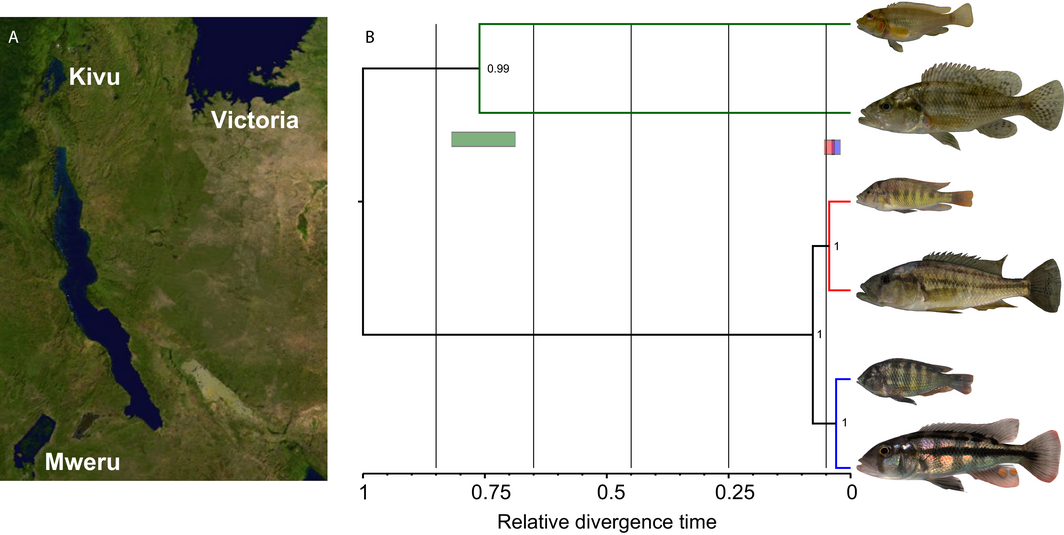
\includegraphics{SpaceGrowth/fig1}
    \caption{\textbf{Growth (OD600) over time of {\em Bacillus safensis} JPL-MERTA-8-2 in space (green) and on Earth (brown).} Values represent the mean of six wells, $\pm$ the standard deviation.}
    \label{SG_fig1}
\end{figure}

It is perhaps no surprise that most built environment-associated bacteria behave very similarly on the ISS as on Earth. After all, the ISS is a home and office of sorts, with environmental conditions very similar to a building on Earth with the exception of gravity. The ISS is maintained at around 22 °C with a relative humidity of around 60% and pressure and oxygen concentrations very close to those at sea level on Earth. Additionally, this experiment did not provide enough time to study the long-term adaptation of bacteria to the environment on board the ISS.

A related project from our lab has examined the microbial community already present on the ISS (Lang et al., unpublished data). Given that the ISS appears to harbor similar microbes to built environments on Earth, we also asked if there were close relatives to our 48 bacteria already present on the ISS. The vast majority (39/48) of our bacterial species were found in the existing microbial community data which is not surprising given the built environment origins of the isolates. This suggests that our data showing these species growing with similar kinetics on space and on Earth is potentially relevant to the biology of the microbial communities already present on the ISS.

